% Copyright (c) 2019-2021, Julien Seguinot (juseg.github.io), Ian Delaney
% Creative Commons Attribution-ShareAlike 4.0 International License
% (CC BY-SA 4.0, http://creativecommons.org/licenses/by-sa/4.0/)

% Alps erosion paper
% ==================

\documentclass[esurf, manuscript]{copernicus}
\usepackage{CJK}  % Japanese text

% custom colours (colorbrewer2.org)
\definecolor{Bu}{cmyk}{1.00,0.45,0.00,0.07}  % Blues
\definecolor{Gn}{cmyk}{1.00,0.20,1.00,0.00}  % Greens
\definecolor{Rd}{cmyk}{0.35,0.95,0.85,0.00}  % Reds
\definecolor{Or}{cmyk}{0.35,0.75,1.00,0.00}  % Oranges
\definecolor{Pu}{cmyk}{0.70,0.80,0.00,0.00}  % Purples
\definecolor{Br}{cmyk}{0.40,0.75,1.00,0.00}  % YlOrBr

% custom commands (remove before submission)
\newcommand{\note}[1]{\textcolor{Or}{\emph{[\textbf{NOTE:} #1]}}}
\newcommand{\todo}[1]{\textcolor{Rd}{\emph{[\textbf{TODO:} #1]}}}

% color links (remove before submission)
\hypersetup{colorlinks, citecolor=Bu, linkcolor=Bu, urlcolor=Bu}

% figures directory
\graphicspath{{../../figures/}}

% document properties
\title{Last glacial cycle glacier erosion potential in the Alps}
\Author[1]{Julien}{Seguinot}
\Author[2]{Ian}{Delaney}
\affil[1]{Independent scholar, Anafi, Greece}
\affil[2]{Institute of Earth Surface Dynamics, University of Lausanne, Switzerland}
\runningtitle{Last glacial cycle glacier erosion potential in the Alps}
\runningauthor{J.~Seguinot and I.~Delaney}


% ======================================================================
\begin{document}
% ======================================================================

\maketitle

\begin{abstract}

    The glacial landscape of the Alps has fascinated generations of explorers,
    artists, mountaineers and scientists with its diversity, including
    erosional features of all scales from high-mountain cirques, to steep
    glacial valleys and large over-deepened basins. Using previous glacier
    modelling results, and empirical inferences of bedrock erosion under modern
    glaciers, we compute a distribution of potential glacier erosion in the
    Alps over the last glacial cycle from 120\,000 years ago to the present.
    %
    Despite large uncertainties pertaining to the climate history of the Alps
    and unconstrained glacier erosion processes, the resulting modelled
    patterns of glacier erosion include persistent features. The cumulative
    imprint of the last glacial cycle shows a very strong localization of
    erosion potential with local maxima at the mouths of major Alpine valleys
    and some other upstream sections where glaciers are modelled to have flown
    with the highest velocity. The potential erosion rates vary significantly
    through the glacial cycle, but show paradoxically little relation to the
    total glacier volume. Phases of glacier advance and maximum extension see a
    localization of rapid potential erosion rates at low elevation, while
    glacier erosion at higher elevation is modelled date from phases of less
    extensive glaciation. The modelled erosion rates peak during deglaciation
    phases, when frontal retreat results in steeper glacier surface slopes,
    implying that climatic conditions that result in rapid glacier erosion
    might be quite transient and specific.
    %
    Our results depict the Alpine glacier erosion landscape as a
    time-transgressive patchwork, with different parts of the range
    corresponding to different glaciation stages and time periods.

\end{abstract}


% ----------------------------------------------------------------------
\introduction
% ----------------------------------------------------------------------

    \begin{figure*}
      \centerline{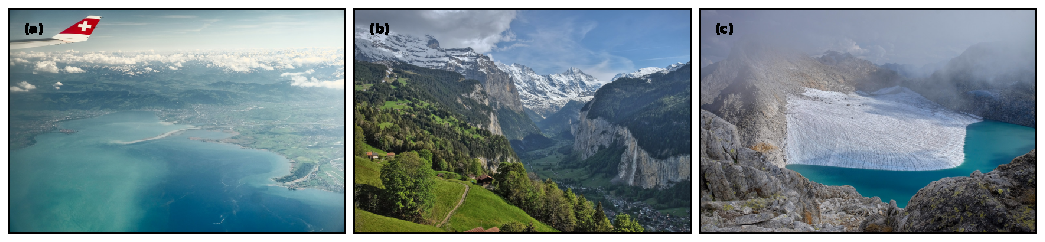
\includegraphics{alpero_landscape}}
      \caption{%
        Alpine glacial erosion landscape diversity.
        \textbf{(a)} Piedmont overdeepening of Lake Constance, ca.~10x50\,km.
        \textbf{(b)} Glacial trough of Lauterbrunnental, ca.~1x10\,km.
        \textbf{(c)} Mountain cirque of Ch\"uebodengletscher, ca.~1x1\,km.}
      \label{fig:landscape}
    \end{figure*}

    The glacial erosion landscape of the Alps has fascinated generations of
    explorers, artists, mountaineers and scientists for centuries. Its cultural
    impact is indeed so far-reaching, that in English, a non-Alpine language,
    the adjective ``alpine'' with non-capital ``a'' is now casually used to
    describe an Alpine-like, glacially modified mountain landscape outside the
    Alps, while the proper noun ``Alps'' has been applied to nick-name
    Alpine-like, glacier eroded mountain ranges in Norway (\emph{Lyngsalpene}),
    New Zealand (Southern Alps), Japan
    (\emph{\begin{CJK}{UTF8}{min}日本アルプス\end{CJK},
    Nihon Arupusu}), and elsewhere.
    %
    Some mountain ranges are predominantly characterised by cirque glaciation
    (e.g. Uinta Mountains), glacial valleys (e.g. Putorana Plateau), or
    large-scale overdeepenings (e.g. Patagonia). But other regions, including
    the Alps \citep[e.g.][Fig.~\ref{fig:landscape}]{Penck.1905}, present a
    higher variety of glacier erosional landforms, whose implications on
    glacial history are yet to be understood.
    The cosmogenic nuclide memory of bedrock erosion provides a more
    quantitative, but equally varied picture of glacier erosion effectiveness
    both within and between glaciated regions \citep{Jansen.etal.2019,
    Steinemann.etal.2020, Steinemann.etal.2021}.

    In the absence of other landforms, glacially eroded topography has
    sometimes been used as a proxy for glacier extent, for instance in
    geomorphological mapping \citep[e.g.,][]{Margold.etal.2011, Fu.etal.2012}.
    Cold-based glaciers, however, have been observed to preserve landforms as
    fragile as sand beaches \citep{Kleman.1994}, leading to the
    reinterpretation of complex glacial landscapes within a binary conceptual
    framework of cold and temperate basal thermal regimes
    \citep{Kleman.etal.2008, Kleman.etal.2010, Fabel.etal.2012, Fu.etal.2013}.
    Nevertheless, it remains unclear how sharp the erosional
    transition to cold-based ice is, and why some glaciated regions show
    preserved periglacial blockfields topped by erratic boulders and others,
    including the Alps, do not \citep{Wirsig.etal.2016, Seguinot.etal.2018}.

    Glacier erosion also likely governs, at least in part,
    the height of mountains \citep{Egholm.etal.2009,Thomson.etal.2010} through
    the ``glacier buzz-saw''. In turn, evidence suggests that increased
    mountain erosion rates coincided with global cooling and Pleistocene
    glaciations from roughly 2.6 million years before present
    \citep{Herman.Champagnac.2016}. However, oceanic isotopic proxies for
    global weathering rates remained constant over this time period
    \citep{Willenbring.Von-Blanckenburg.2010}. Examination of contemporary
    erosion rates across different climates suggests that increased temperatures
    in glaciated regions lead to higher erosion rates and that erosion rates
    may have increased towards present \citep{Koppes.Montgomery.2009,
    Koppes.etal.2015, Fernandez.etal.2016}. However, understanding the link
    between climate and glacier erosion in the sedimentary record remains
    difficult due to time scale biases \citep{Ganti.etal.2016} and the
    non-linear relationship  between atmospheric temperature and erosion
    \citep[e.g.,][]{Anderson.etal.2012,Mariotti.etal.2021}.
    \todo{shorten this paragraph.}

    Observing and quantifying the long-term glacier erosion and sedimentation
    processes has been a challenge, and two general methods have been adopted
    to quantify erosion \citep{Alley.etal.2019}. Physically-based models
    describe quarrying process and abrasion of bedrock by debris-laden ice
    \citep[e.g.,][]{Alley.etal.1997, Iverson.2012, Beaud.etal.2014}. Describing
    the processes physically provides a basis for understanding erosion
    processes \citep{Hallet.1979, Ugelvig.etal.2018} and yields insight into
    the formation of glacial landforms, such as tunnel valleys and eskers
    \citep{Beaud.etal.2018, Hewitt.Creyts.2019}. Yet, these models prove
    difficult to implement in many cases due to the large number of poorly
    constrained parameters and processes, i.e. water pressure fluctuations and
    subglacial debris concentration \citep[e.g.,][]{Hallet.1979, Seguinot.2008,
    Ugelvig.etal.2018}.

    Instead, empirical relationships between glacier sliding and erosion can
    represent erosional quantities well and can recreate important glacial
    landforms \citep[e.g.,][]{Harbor.etal.1988, Macgregor.etal.2000}.
    For instance, \citet{Humphrey.Raymond.1994} correlated temporal variations
    in ice velocity and suspended sediment load during a surge of Variegated
    Glacier to establish a linear erosion law.
    \citet{Koppes.etal.2015} quantified sediment
    yields in 15~Patagonian and Antarctic Peninsula fjords, concluding at a
    predominant control of surface air temperature on rapid glacier erosion and
    calibrating a near-square-law from glacier velocity to erosion rate.
    \citet{Herman.etal.2015} collected suspended sediment samples for 5~months
    in the outlet stream of Franz-Josef Glacier, mapped their chemical
    composition to geologic zones of distinctive glacier speed, and also
    concluded to a near-square relationship between basal sliding and glacier
    erosion.
    \citet{Cook.etal.2020} assembled a global compilation of erosion rates for
    38~glaciers, showing a predominant role of glacier sliding velocity over
    climate variables, yet concluding at a sub-linear relationship to erosion.

    Here, the non-linear erosion law by \citet{Koppes.etal.2015} is applied to
    previously published model results \citep{Seguinot.etal.2018} and the
    patterns of modelled erosion potential and cumulative last glacial cycle
    erosion
    potential are analysed. We examine the glaciological conditions that cause
    erosion and discuss the implications of these conditions on understanding
    the relationship between climate and glacier erosion. Despite aggregated
    uncertainties on paleoclimate, glacier flow and glacier erosion processes,
    out results provide insights into the diversity of the Alpine glacial
    erosion landscape.


% ----------------------------------------------------------------------
\section{Methods}
% ----------------------------------------------------------------------

% -- -- -- -- -- -- -- -- -- -- -- -- -- -- -- -- -- -- -- -- -- -- -- -
\subsection{Ice sheet modelling}
% -- -- -- -- -- -- -- -- -- -- -- -- -- -- -- -- -- -- -- -- -- -- -- -

    The ice-sheet model set-up was presented in an earlier publication
    \citep{Seguinot.etal.2018} and is briefly summarized here. The simulations
    were conducted using the Parallel Ice Sheet Model (PISM, development
    version~e9d2d1f), an open-source, finite-difference, shallow-ice and
    shallow-shelf model \citep{PISM-authors.2017}. Our setup includes
    temperature and water-content dependent creep, pseudo-plastic basal
    sliding, bedrock isostatic deformation under the ice
    load, and a~positive degree-day (PDD) surface mass balance model. The model
    is initialized with assumed present-day ice thickness and bedrock topography
    from SRTM \citep{Jarvis.etal.2008},
    ice and bedrock temperature at 120\,ka (thousand years before the present),
    and is run to the present. The ice-sheet model physical parameters are listed
    in the earlier open-access publication \citep{Seguinot.etal.2018}, and the
    complete list of PISM
    parameters is stored in long-term archived model output metadata for the
    present study \citep{Seguinot.2021}, and for the earlier publication
    \citep{Seguinot.2020, Seguinot.2020a}.

    Climate forcing is provided by a~monthly climatology from interpolated
    observational data \citep[WorldClim;][]{Hijmans.etal.2005} and the European
    Centre for Medium-Range Weather Forecasts Reanalysis Interim
    \citep[ERA-Interim;][]{Dee.etal.2011}, amended with temperature changes
    from the European Project for Ice Coring in Antarctica
    \citep[EPICA;][] {Jouzel.etal.2007}, and time-dependent paleo-precipitation
    reductions \citep{Huybrechts.2002}. Lower-resolution runs based on
    alternative paleoclimate scenarios \citep{Seguinot.etal.2018}, forced by
    temperature changes from the the Greenland Ice Core Project
    \citep[GRIP;][]{Dansgaard.etal.1993} and and an oceanic sediment core from
    the Iberian margin \citep[MD01-2444;][]{Martrat.etal.2007}, are analyzed
    in the discussion part (Sect.~\ref{sec:sensitivity}).

% -- -- -- -- -- -- -- -- -- -- -- -- -- -- -- -- -- -- -- -- -- -- -- -
\subsection{Erosion law}
% -- -- -- -- -- -- -- -- -- -- -- -- -- -- -- -- -- -- -- -- -- -- -- -

    Modelled erosion rates, $\dot{e}$, are calculated from the modelled basal
    velocities, $u_\mathrm{b}$, using a empirical erosion power-law,
    %
    \begin{equation}
        \dot{e} = K_\mathrm{g} u_\mathrm{b}^l ,
    \end{equation}
    %
    where $K_g = 5.2\times 10^{-11}\,m^{1-l}\,a^{l-1}$ and $l = 2.34$ are
    empirical constants calibrated on quantified fjord sediment yields and
    velocities from 15~Patagonian and Antarctic Peninsula tidewater glaciers
    \citep[using the full dataset from][including outliers]{Koppes.etal.2015}.
    We discuss the role of alternative values of
    $K_\mathrm{g}$ and $l$ in the discussion part (Sect.~\ref{sec:powerlaws}).

    Our approach does not account for feedbacks of glacier erosion onto
    bedrock topography and, then onto, ice dynamics
    \citep[e.g.,][]{Anderson.etal.2012}. Furthermore, we do not account for the
    downstream advection of debris \citep[e.g.,][]{Anderson.Anderson.2016},
    or fluvial transport of subglacial sediment \citep{Delaney.etal.2019}.
    Instead we assume that eroded material is instantly transported out of the
    system, thus neglegting its role in shielding the bedrock from glacier
    erosion in zones of temporary storage \citep{Preusser.etal.2010}. Neither
    do we account for differences in erosion effectiveness on different
    lithologies or erosion from subglacial and interglacial hydrologic
    processes. For the aforementioned reasons, we refer to the above computed
    rates, $\dot{e}$, as ``potential erosion rates''.

    Secondly, we compute the time-integrated glacier erosion rate,
    %
    \begin{equation}
        e =  K_\mathrm{g} \int u_\mathrm{b}^l dt,
    \end{equation}
    %
    and refer to it as the ``cumulative erosion potential''. The integration
    is numerically approximated using a time-step of 10\,a in the
    main simulation, and 100\,a in the alternative climate scenarios runs.
    Note that in the above formula with an exponent, $l$,
    higher than one, the cumulative erosion potential has a greater dependency
    on the basal ice dynamics, $u_\mathrm{b}$, than the duration of glacier
    cover.


% ----------------------------------------------------------------------
\section{Results}
% ----------------------------------------------------------------------

% -- -- -- -- -- -- -- -- -- -- -- -- -- -- -- -- -- -- -- -- -- -- -- -
\subsection{Cumulative erosion}
% -- -- -- -- -- -- -- -- -- -- -- -- -- -- -- -- -- -- -- -- -- -- -- -

    \begin{figure*}
      \centerline{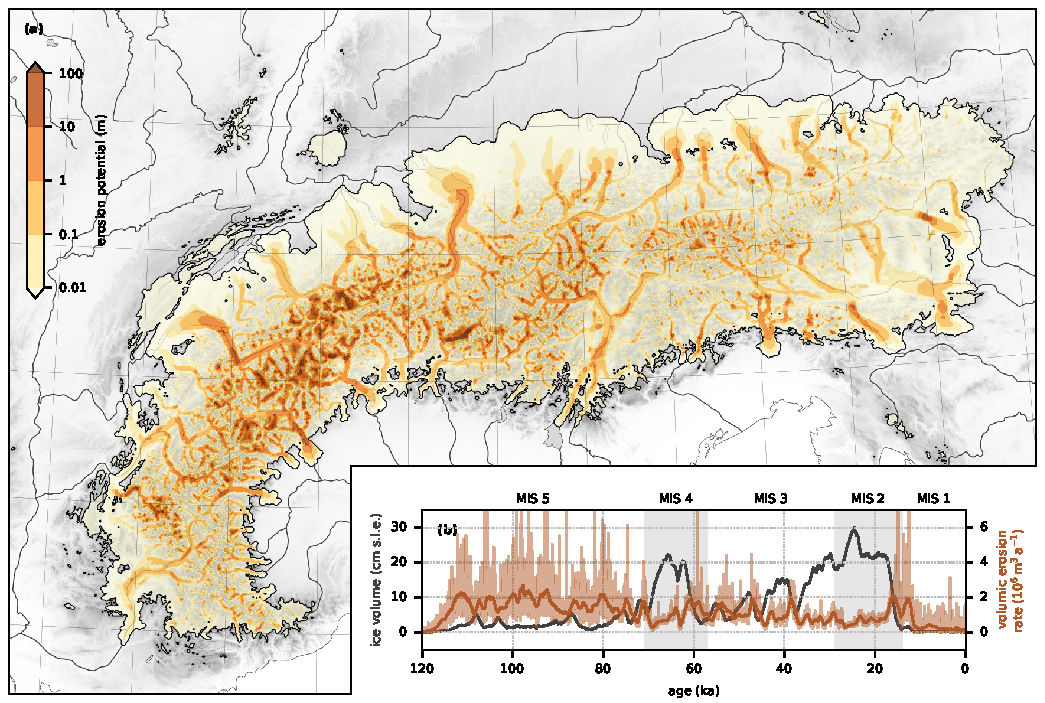
\includegraphics{alpero_cumulative}}
      \caption{%
        \textbf{(a)} Modelled cumulative (time-integrated) glacial erosion
          potential over the last glacial cycle and geomorphological
          reconstruction of Last Glacial Maximum Alpine glacier extent for
          comparison \citep[solid red line,][]{Ehlers.etal.2011}.
          The background maps consists of the initial basal topography from
          SRTM \citep{Jarvis.etal.2008} and Natural Earth Data
          \citep{Patterson.Kelso.2017}.
        \textbf{(b)} Modelled total ice volume in centimetres of sea-level
          equivalent (cm~s.l.e., black), annual (domain-integrated) potential
          erosion volume (light brown) and its 1-ka running mean (dark brown).
          Shaded gray areas indicate the timing for MIS~2 and~4
          \citep{Lisiecki.Raymo.2005}.
        \todo{hatches on all plots.}}
        \label{fig:cumulative}
    \end{figure*}

    The modelled cumulative (time-integrated) glacial erosion potential
    (Fig.~\ref{fig:cumulative}a) varies by several orders of magnitude
    from insignificant to hundred-metres-scale erosion potential. Its spatial
    patterns show a very strong localization along the Alpine valleys, with
    local maxima occurring both at
    the Alpine gates where ice flow transited from valley to piedmont glaciers,
    and further upstream where the valley slopes increase. While mountain
    cirque glaciers and relevant erosion processes may not be captured by the
    model physics and horizontal resolution, high
    cumulative erosion potential also occurs near the valley heads.
    There is a general tendency for higher cumulative erosion in the
    north-western Alps where the input winter precipitation is higher
    \citep[WorldClim, Fig.~1h in][]{Seguinot.etal.2018} and the glacial relief
    more pronounced in the topography.

% -- -- -- -- -- -- -- -- -- -- -- -- -- -- -- -- -- -- -- -- -- -- -- -
\subsection{Temporal evolution}
% -- -- -- -- -- -- -- -- -- -- -- -- -- -- -- -- -- -- -- -- -- -- -- -

    \begin{figure}
      \centerline{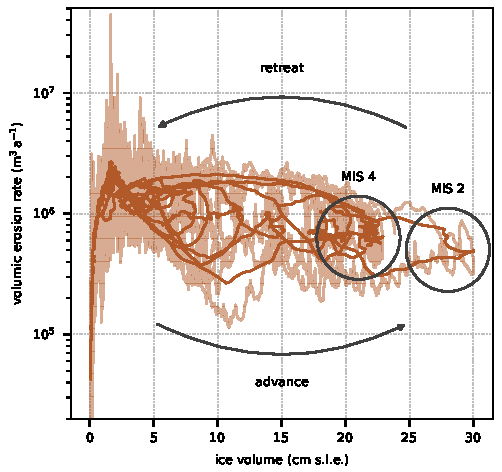
\includegraphics{alpero_evolution}}
      \caption{%
        Modelled annual (domain-integrated) potential erosion volume (light
        curves) and its 1-ka running mean (dark curves) in relation to the
        modelled total ice volume in centimetres of sea-level equivalent. Blue
        indicates increasing ice volume and brown decreasing ice volume.}
      \label{fig:evolution}
    \end{figure}

    The modelled annual (domain-integrated) potential glacial erosion volume
    does not systematically correlate with the modelled total ice volume
    (Fig.~\ref{fig:cumulative}b). Except for the onset and termination of the
    glacial cycle were ice volume is low and sliding processes unlikely to be
    captured by the model resolution, a comparison between the modelled ice
    volume and the modelled annual erosion volume shows no single relation
    between these two quantities (Fig.~\ref{fig:evolution}). After significant
    ice volume has been reached, there is a general tendency for slower erosion
    during periods of extensive glaciation (Fig.~\ref{fig:evolution}). However,
    the domain-integrated erosion volume is modelled to be consistently higher
    (by a factor 2 to 10) during periods of decreasing ice volume, than during
    periods of increasing ice volume (Fig.~\ref{fig:evolution}).

% -- -- -- -- -- -- -- -- -- -- -- -- -- -- -- -- -- -- -- -- -- -- -- -
\subsection{Spatial migration}
% -- -- -- -- -- -- -- -- -- -- -- -- -- -- -- -- -- -- -- -- -- -- -- -

    \begin{figure*}
      \centerline{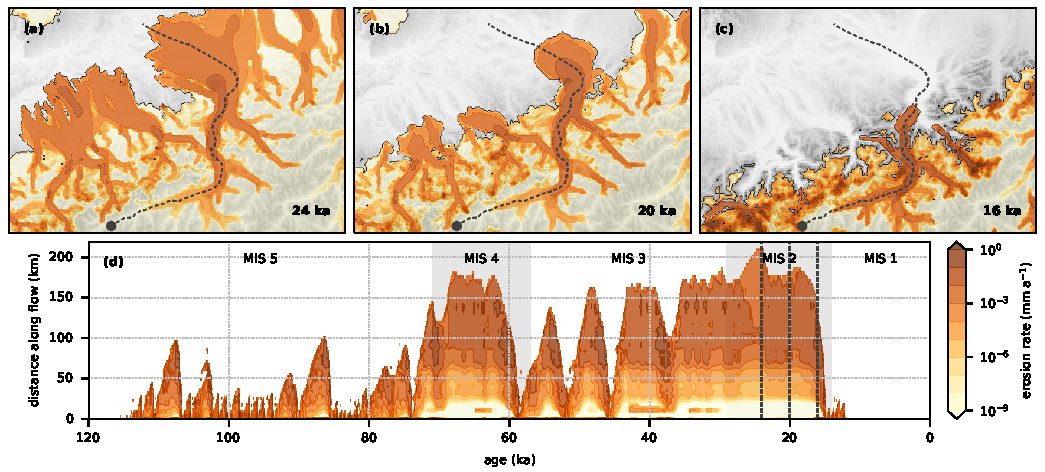
\includegraphics{alpero_transects}}
      \caption{%
        \textbf{(a--d)} Modelled instantaneous potential erosion rate of the
          Rhine Glacier for selected glacier advance and retreat ages, and the
          final model state for topographic reference.
        \textbf{(e)} Interpolated instantaneous potential erosion rate along a
          Rhine Glacier transect (upper panels dashed line) for the entire last
          glacial cycle.}
      \label{fig:transects}
    \end{figure*}

    \begin{figure*}
      \centerline{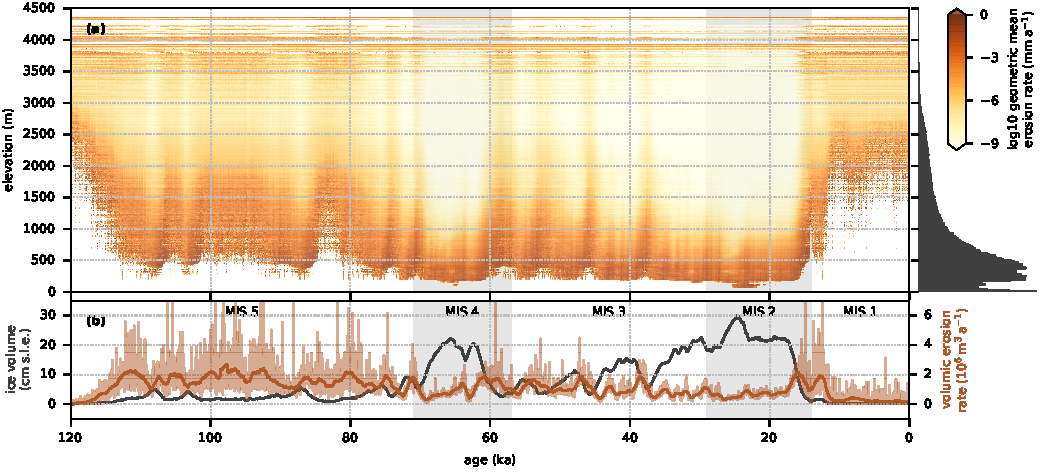
\includegraphics{alpero_hypsogram}}
      \caption{%
        \textbf{(a)} Potential erosion rate ``hypsogram'', showing the
          geometric mean of (non-zero) modelled rates in 10-m elevation bands
          across the entire model domain and its time evolution.
        \textbf{(b)} Distribution of model domain bedrock topography (grey
          bars) and glaciated topography (blue bars) in 100-m elevation bands,
          and the corresponding cumulative potential erosion volume (brown
          line).
        \textbf{(c)} Same as Fig.~\ref{fig:cumulative}b.
        \todo{fix labels, test hatching below a minimum number of grid cells}}
      \label{fig:hypsogram}
    \end{figure*}

    A closer look at the Rhine Glacier, one of the paleo-ice sheet's largest
    outlets, reveals a spatial migration of the modelled rapid erosion areas.
    During stages of glacier advance and maximum extension, erosion is modelled
    to be under 1\,mm\,a$^{-1}$ and restricted the lower parts of the
    catchment, while much of the intra-montane Alps \citep[modelled to be
    largely cold-based, Fig.~6c in][]{Seguinot.etal.2018} experience
    insignificant erosion potential (Fig.~\ref{fig:transects}a and~b). The
    potential erosion rates both increase and propagate inwards during periods
    of glacier retreat (Fig.~\ref{fig:transects}c and~e).

    The results found on the Rhine Glacier catchment can be generalized to the
    entire model domain by using (present-day) bedrock altitude as a proxy for
    along-flow distance (Fig.~\ref{fig:hypsogram}). Thus more generally,
    periods of modelled increasing and maximum ice volume correspond to lower
    values for elevation-aggregated potential erosion rates, with significant
    erosion potential
    restricted to lower elevations. On the opposite, periods of modelled
    decreased ice volume correspond to higher local modelled erosion rates and
    more extensive rapid erosion potential into higher-elevation areas
    (Fig.~\ref{fig:hypsogram}).


% ----------------------------------------------------------------------
\section{Discussion}
% ----------------------------------------------------------------------

% -- -- -- -- -- -- -- -- -- -- -- -- -- -- -- -- -- -- -- -- -- -- -- -
\subsection{Climate sensitivity}
\label{sec:sensitivity}
% -- -- -- -- -- -- -- -- -- -- -- -- -- -- -- -- -- -- -- -- -- -- -- -

    \begin{figure*}
      \centerline{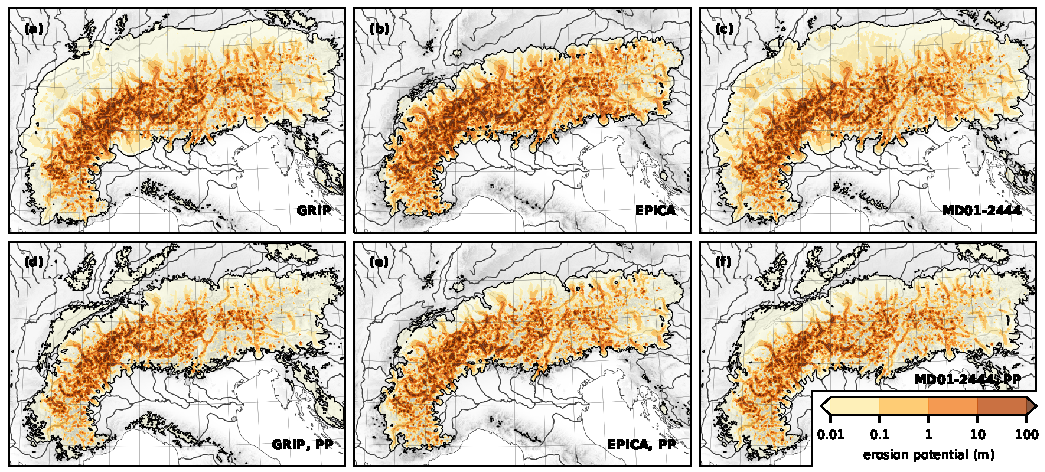
\includegraphics{alpero_sensitivity}}
      \caption{%
        Modelled cumulative glacial erosion potential over the last glacial
        cycle using three different paleo-temperature histories from
        \textbf{(a, d)} the Greenland Ice Core Project
        \citep[GRIP;][]{Dansgaard.etal.1993}, \textbf{(b, e)} the European
        Project for Ice Coring in Antarctica \citep[our default,
        EPICA;][]{Jouzel.etal.2007}, and \textbf{(c, f)} an oceanic sediment
        core from the Iberian margin \citep[MD01-2444;][]{Martrat.etal.2007},
        and both \textbf{(a--c)} without and \textbf{(d--f)} with
        paleo-precipitation reductions \citep[cf.][]{Seguinot.etal.2018}.}
      \label{fig:sensitivity}
    \end{figure*}

    Different paleoclimate forcing scenarios lead to different modelled
    glaciation histories \citep[cf.][]{Seguinot.etal.2018} and thus different
    results in terms of glacial cycle cumulative erosion
    potential (Fig.~\ref{fig:sensitivity}). Scenarios including higher
    (constant, present-day) input precipitation rates yield generally higher
    modelled ice discharge and thus higher
    erosion potential (Fig.~\ref{fig:sensitivity}a--c), while scenarios
    including paleo-precipitation reductions (Fig.~\ref{fig:sensitivity}d--f),
    including our default high-resolution run
    (Fig.~\ref{fig:cumulative}), yield a smaller erosion potential.

    The spatial pattern of modelled time-integrated erosion is nevertheless
    generally consistent across the paleoclimate scenarios tested,
    despite variations in the glaciation maximum extent
    (\citealp[Fig.~3 in][]{Seguinot.etal.2018}; Fig.~\ref{fig:sensitivity}).
    It should be noted, however, that all runs presented here show a systematic
    bias with excessive glacier cover in the Eastern Alps and a diminished
    glacier extent in the Western Alps (Fig.~\ref{fig:cumulative}a; further
    discussed in \citealp{Seguinot.etal.2018}). Thus the modelled patterns of
    erosion potential certainly includes a similar bias. However, uncertainties
    due to paleoclimate appear minor in regard to the much larger uncertainties
    affecting the choice of erosion law.

% -- -- -- -- -- -- -- -- -- -- -- -- -- -- -- -- -- -- -- -- -- -- -- -
\subsection{Choice of erosion law}
\label{sec:powerlaws}
% -- -- -- -- -- -- -- -- -- -- -- -- -- -- -- -- -- -- -- -- -- -- -- -

    \begin{figure*}[t]
      \centerline{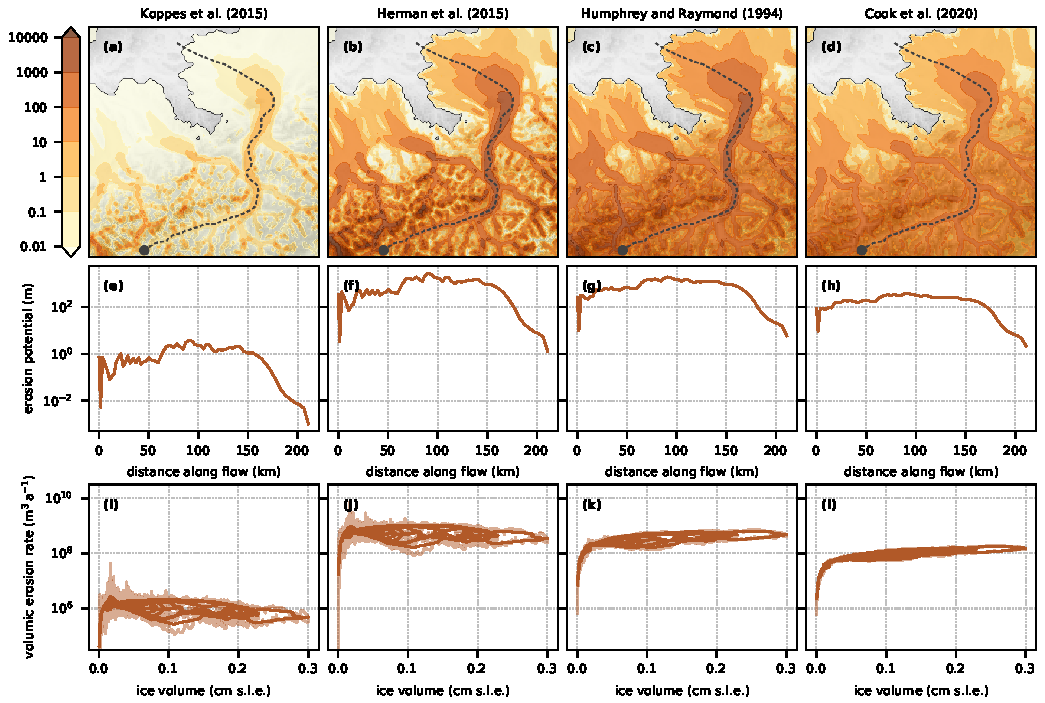
\includegraphics{alpero_powerlaws}}
      \caption{%
        Modelled cumulative (time-integrated) glacial erosion potential for
        three different erosion laws published by
        \textbf{(a)} \citet{Koppes.etal.2015},
          ${5.2 \times 10^{-8} u_\mathrm{b}^{2.34}}$ (same as
          Fig.~\ref{fig:cumulative}a but with a different colour scale),
        \textbf{(b)} \citet{Herman.etal.2015},
          ${2.7 \times 10^{-7} u_\mathrm{b}^{2.02}}$,
        \textbf{(c)} \citet{Humphrey.Raymond.1994},
          ${1 \times 10^{-4} u_\mathrm{b}^{1}}$, and
        \textbf{(d)} \citet{Cook.etal.2020},
          ${1.665 \times 10^{-1} u_\mathrm{b}^{0.6459}}$.
        \textbf{(e-h)} Corresponding modelled cumulative glacial erosion
          potential along a Rhine Glacier transect (upper panels dashed line), and
        \textbf{(i-l)} corresponding modelled evolution of annual
        (domain-integrated) erosion volume (light brown) and 1-ka
        running mean (dark brown) in relation to modelled total ice volume in
        centimetres of sea-level equivalent (as in Fig.~\ref{fig:evolution}a).}
      \label{fig:powerlaws}
    \end{figure*}

    The choice of erosion law significantly impacts the results
    (Fig.~\ref{fig:powerlaws}). Our default, based on quantified
    sediment yields from Patagonian and Antarctic Peninsula tidewater glaciers
    \citep[${\dot{e}=5.2\times10^{-8}u_\mathrm{b}^{2.34}}$,][]{Koppes.etal.2015}
    yields a moderate and strongly localized cumulative erosion potential
    (Figs~\ref{fig:cumulative} and~\ref{fig:powerlaws}a). The erosion law
    based on measured suspended sediment load from Franz-Joseph Glacier
    \citep[${\dot{e}=2.7\times10^{-7}u_\mathrm{b}^{2.02}}$,][]{Herman.etal.2015}
    also yields a strongly localized, and yet much higher, modelled erosion
    potential (Fig.~\ref{fig:powerlaws}b). The erosion law based on measured
    suspended sediment load during a surge of Variegated Glacier
    \citep[${\dot{e}=1\times10^{-4}u_\mathrm{b}^{1}}$,][]{Humphrey.Raymond.1994}
    results in similarly high values, but a less localized pattern of cumulative
    erosion potential (Fig.~\ref{fig:powerlaws}c). Finally, The erosion law
    based on a global compilation of glacier velocities and erosion rates
    \citep[${\dot{e}=1.665\times10^{-1}u_\mathrm{b}^{0.6459}}$,][]{Cook.etal.2020}
    yields an even flatter pattern of cumulative erosion potential
    (Fig.~\ref{fig:powerlaws}d).

    With a total Pleistocene glacial relief on the order of a kilometre
    \citep{Preusser.etal.2011, Valla.etal.2011}, a cumulative glacial erosion
    for the last glacial cycle in the order of 10--100\,m can be expected.
    However, none of the tested erosion power-laws fall within this range.
    Instead, the erosion law calibrated on tidewater glaciers
    \citep{Koppes.etal.2015} yields cumulative erosion in the Rhine Valley in
    the orders of metres, while the three erosion laws based on terrestrial
    glaciers \citep{Humphrey.Raymond.1994, Herman.etal.2015, Cook.etal.2020},
    result in kilometre-scale integrated erosion potential. During the Last
    Glacial Maximum and much of the last glacial cycle, Alpine paleoglaciers
    were closer in size, slope (an important parameter as we argue in the next
    section), and climatic context to the present-day glaciers of
    Patagonia and the Antarctic Peninsula \citep{Koppes.etal.2015} than to
    Franz-Joseph Glacier \citep{Herman.etal.2015} and many of the glaciers
    included in the global compilation by \citet{Cook.etal.2020}.
    This may help to explain why the reality appears to fall in-between the
    tested erosion laws.

    That said, the magnitude of the modelled erosion rates can hardly be used
    as a criteria to rule out this or that erosion law for the glacial Alps.
    While sliding is here modelled by a pseudo-plastic law based on
    till dilatation under high water pressure \citep{Tulaczyk.etal.2000},
    empirical erosion rules are thought to be a proxy for glacier abrasion
    (cf.~\citealp{Hallet.1979}; and possibly plucking) of a glacier flowing
    over a hard bed. Current erosion rates in the Alps strongly vary depending
    on the substratum \citep{Steinemann.etal.2020, Steinemann.etal.2021}, and
    it is arguable that a layer of till and proglacial sediments may have
    armored the glacier bed from erosion for at least parts of the glacial
    cycle. Thus, given the lack of data to constrain the erosion rule, it can
    not be excluded that a linear or sub-linear erosion law
    \citep[e.g.,][]{Cook.etal.2020} would lead to a less localized pattern of
    erosion (Fig.~\ref{fig:powerlaws}c and~d), and a stronger correlation
    between modelled ice volume and erosion (Fig.~\ref{fig:powerlaws}k and~l).
    \todo{discuss Koppes without outliers}

    The modelled pattern of erosion potential depends on PISM glacier physics
    and sliding model parameters. In particular, the pseudo-plastic sliding law
    exponent \citep[$q=0.25$ in][]{Seguinot.etal.2018} controls the sharpness
    of the transition between adherent and decoupled basal conditions. Recent
    ensemble validation of Antarctic Ice Sheet glacial-cycle simulations
    against geological and present-day observations \citep{Albrecht.etal.2020,
    Albrecht.etal.2020a} support a higher value of $q=0.75$, and thus a
    sliding law closer to linear, which would perhaps result in a smoother
    distribution of sliding velocity and erosion potential. Lateral stress
    gradients missing from the shallow-shelf approximation stress balance could
    also contribute to moderate sliding velocity in narrow troughs
    \citep{Herman.etal.2011, Egholm.etal.2012, Egholm.etal.2012a,
    Pedersen.etal.2014}. \todo{check these references}.

    Because of the intrinsically large variations in modelled glacier sliding
    velocities yield cumulative glacial-cycle erosion two to three orders of
    magnitude higher in the Alpine valleys than near the mountain tops
    (Fig.~\ref{fig:powerlaws}d), we argue that the modelled highly localized
    pattern of erosion potential is qualitatively robust. This pattern, and
    the lithologic variations in bedrock erodability, may explain
    order-of-magnitude variation of glacier erosion rates observed in the
    cosmogenic nuclide record \citep{Jansen.etal.2019, Steinemann.etal.2020,
    Steinemann.etal.2021}.


% -- -- -- -- -- -- -- -- -- -- -- -- -- -- -- -- -- -- -- -- -- -- -- -
\subsection{Climate control on erosion}
% -- -- -- -- -- -- -- -- -- -- -- -- -- -- -- -- -- -- -- -- -- -- -- -

    \begin{figure}
      \centerline{\includegraphics{alpero_basaldrag}}
      \caption{%
        \textbf{(a)} Modelled basal and surface topographies interpolated along
        the Rhine Glacier during glacier advance (36\,ka), maximum extent
        (24\,ka) and retreat (16\,ka, using the same transect as in
        Fig.~\ref{fig:basaldrag}).
        \textbf{(b)} Interpolated yield stress in the pseudo-plastic sliding law
        (dotted lines) and magnitude of the basal shear stress (basal drag,
        solid lines), both normalized against the ice overburden pressure.
        Basal drag values greater than yield stress result in glacier sliding
        \citep[cf.][for model physics]{Seguinot.2014, Seguinot.etal.2016}.}
      \label{fig:basaldrag}
    \end{figure}

    The modelled, domain-integrated glacier erosion volume does not increase
    together with ice volume. On the opposite, periods of ice advance and
    maximum glaciation correspond to comparatively slow erosion potential
    (Figs.~\ref{fig:cumulative} and~\ref{fig:evolution}).
    This result may seem paradoxical, and is modulated in a limited extent by
    the exponent, $l$, in the erosion rule (Fig.~\ref{fig:powerlaws}).
    Nevertheless, it may explain why some areas covered during glacial maxima
    only, such as some valleys on the southern side of the Alps, appear to have
    experienced only little glacial modification of their topography.
    During deglaciation periods, increased surface melt at low elevations
    results in a steepened topographic profile (Figs.~\ref{fig:basaldrag}a),
    as observed and further expected on currently retreating glaciers
    \citep{Huss.etal.2010, Zekollari.Huybrechts.2015}.
    The buttress formed by the glacier foot against gravitational forces is
    reduced, causing an increase in the magnitude of the basal shear stress
    (basal drag) relative to the ice overburden pressure, and an increase in
    the area where sliding and thus, erosion, can occur
    (Figs.~\ref{fig:basaldrag}b).

    This result is corroborated by a recent denudation record from the
    Mediterranean Alps, which includes an increase in glacier erosion in the
    Var Valley, roughly at 25\,ka following an extended period of low
    denudation rates \citep{Mariotti.etal.2021}. While that increase in
    erosion predates the increase observed in our study (ca.~15\,ka;
    Fig.~\ref{fig:evolution}), it demonstrates that climatic conditions
    over which glacier erosion occurs are relatively specific and likely
    transient. Other field-based studies have evidenced increased glacier
    erosion and pro-glacial sedimentation during the current deglaciation period
    \citep[e.g.,][]{Koppes.Montgomery.2009, Micheletti.Lane.2016,
    Lane.etal.2017, Bendixen.etal.2017}. This increase has often been
    attributed to higher meltwater availability, promoting sediment transport
    \citep{Delaney.Adhikari.2020}, enhanced glacier sliding
    \citep{Herman.etal.2011}, and hydrofracturing, i.e.~plucking
    \citep{Hallet.1996, Ugelvig.etal.2018, Hildes.etal.2004}.

    But importantly, these hydrological processes are not included in our
    model, so that deglaciation surface meltwater is assumed to instantly exit
    the glacier with no effect on glacier dynamics \citep[cf.][for comparison]
    {Werder.etal.2013, Iverson.2012, Ugelvig.etal.2018}. The enhanced glacier
    velocity during periods of ice retreat is here modelled to result from
    changes in glacier geometry alone (Figs.~\ref{fig:basaldrag}b).
    Observed feedbacks between
    surface meltwater and basal sliding, not included in the model, presumably
    further accelerated erosion during deglaciation \citep{Herman.etal.2011}.
    Furthermore, we omit the fluvial transport of sediment, which could well
    increase sediment discharge and erosion with increased melt, so long as
    additional sediment remains available \citep{Delaney.Adhikari.2020}. Rapid
    glacier erosion can be expected to accompany the ongoing 21st-century
    deglaciation, especially for the ice sheets of Greenland and
    Antarctica where polythermal and cold-based glaciers are warming and
    sliding may increase \citep[e.g.,][]{Moon.etal.2012, Mouginot.etal.2014,
    Overeem.etal.2017}.

% -- -- -- -- -- -- -- -- -- -- -- -- -- -- -- -- -- -- -- -- -- -- -- -
\subsection{Age of the glacial landscape}
% -- -- -- -- -- -- -- -- -- -- -- -- -- -- -- -- -- -- -- -- -- -- -- -

    In many places throughout the Alps, significant modelled cumulative erosion
    occurs far inside the Alpine valleys (Fig.~\ref{fig:cumulative}). However,
    the potential erosion patterns experience spatial shifts through the
    glacial cycle (Fig.~\ref{fig:transects}), so that high-altitude rapid
    erosion is not modelled to date from expansive glaciation stages, but
    instead from stages of intermediate glacier cover
    \citep[Fig.~\ref{fig:hypsogram};][]{Barr.etal.2019}.

    For instance, low-elevation piedmont over-deepened basins such as Lake
    Constance (Fig.~\ref{fig:landscape}), Lake Geneva and Lake Maggiore are
    here modelled to be the product of extensive Last Glacial Maximum-like
    glaciations. Other modelling work suggests that features such as these
    likely form when water can access the glacier bed and encourage glacier
    sliding and, thus, erosion \citep{Herman.etal.2011}. The model herein does
    not include subglacial hydrology, yet the role of climate warming to
    increasing glacier erosion to the lower elevations remains evident
    (Fig.~\ref{fig:hypsogram}).
    Alpine terrain with elevations above 1000\,m are modelled to
    experience virtually no erosion from 35 to 18\,ka BP
    (Fig.~\ref{fig:hypsogram}), so that many of the most spectacular,
    intermediate-elevation glacial valleys of the Alps as Lauterbrunnental
    (Fig.~\ref{fig:landscape}), Haslital (Upper Aare) or Bout du Monde (Upper
    Giffre) would date from periods of intermediate glacier extension.

    The validity of the model results at high elevation is discussable.
    Cristalline massifs such as the Ecrins, Gran Paradiso, Monte Rosa, Aare,
    \"Otztal and Tauern Massifs locally exhibit a strikingly high erosion
    potential. However, the computation of glacier flow velocities on such
    steep surfaces is strongly limited by the model horizontal resolution of
    1\,km, the shallow-ice glacier flow physics \citep{Imhof.etal.2019}, and
    PISM's current mass-conservation heuristics \citep{Imhof.2021}. Besides,
    bergschrund (rimaye) processes likely to dominate interglacial cirque
    erosion at such altitudes \citep{Sanders.etal.2012} are not captured by the
    velocity-based glacier erosion power-laws. Nevertheless,
    the lack of rapid erosion at high elevations for much of the modelled
    glacial cycle (Fig.~\ref{fig:hypsogram}) implies that the highest mountain
    cirques such as Ch\"uebodensee (Fig.~\ref{fig:landscape}) would have formed
    over interglacial periods, when glaciers are confined to high terrain
    \citep{Barr.etal.2017, Barr.etal.2019}. Similar processes also occur on
    Himalayan glaciers and may limit erosion for the high elevation portion of
    that mountain range during cold periods as well, failing to offset uplift
    rates \citep{Harper.Humphrey.2003}. Over longer timescales, though, the
    vertical distribution of erosion rates also depends on the erosional
    modification of topography \citep{Sernai.etal.2013}.

    Finally, the time-transgressive nature of the modelled glacial erosion
    rates hint at a new explanation for the Alpine glacier trim-line and lack
    of cold-based glaciation evidence. Due to their geographic location in the
    mid-latitudes, and their steep topographic gradient, the Alps appear as a
    mountain range that hosted glaciers of various sizes throughout the varying
    climate of the Quaternary, resulting in a transgressive localization of
    glacier erosion throughout their elevational range, from the piedmont
    during glacial maxima, to the highest cirques during interglacial periods.
    The Alpine trim-line, in this case, would neither correspond to the upper
    reach of the Last Glacial Maximum glaciers \citep[e.g.,][]{Kelly.etal.2004},
    nor to an englacial temperate-ice boundary \citep{Coutterand.2010,
    Seguinot.etal.2018}, but to a time-transgressive upper limit of erosion from
    advancing and retreating glaciers on steep terrain.


% ----------------------------------------------------------------------
\conclusions
% ----------------------------------------------------------------------

    Due to compounded uncertainties regarding paleoclimate, glacier sliding and
    erosion processes, our quantitative results are very likely inaccurate.
    However, we draw the following qualitative conclusions:
    \begin{itemize}
      \item The non-linear physics of glacier deformation and sliding, combined
        with non-linear empirical erosion laws, results in a very strong
        localization of rapid glacier erosion in regions of fast flow.
      \item This high spatio-temporal variability hints at a complex
        relationship between climate and glacier erosion, so that a highly
        variable response of glacier erosion to climate should be expected.
      \item Increased gravitational drag due to surface profile steepening
        provides a mechanism
        for accelerated erosion during deglaciation periods, irrespective of
        surface meltwater penetration to the glacier bed.
      \item If a non-linear glacier erosion law is used, the climate-induced
        slowdown of erosion counterbalances glacier expansion, so that
        Alpine-wide glacier erosion volumes do not correlate with the ice volume.
      \item Rapid glacier erosion is restricted to low elevation during stages
        of glacier advance and maximum glaciation, but propagates up-valley to
        higher elevations during periods of glacier retreat.
      \item The diversity of the Alpine glacier erosion landscape appears to
        be the time-transgressive signature of a variety of glacial stages
        ranging from pan-Alpine ice sheets to modern-style mountain glaciers.
    \end{itemize}


% ----------------------------------------------------------------------
% Acknowledgements
% ----------------------------------------------------------------------

\codedataavailability{%
    PISM is available as open-source software (http://pism-docs.org).
    Time and domain-aggregated erosion variables such as used in the figures is
    available for the four presented erosion power-laws
    (\doi{10.5281/zenodo.4495419}). Other model output variables were
    previously made available (\doi{10.5281/zenodo.3604174},
    \doi{10.5281/zenodo.3604142}).}

\videosupplement{
    Animations made available online show the modelled glacier erosion rates
    (\url{https://vimeo.com/503162771}), and their evolving relationship with
    ice volume (\url{https://vimeo.com/512478926}) and bedrock
    altitude (\url{https://vimeo.com/512479008}).}

\authorcontribution{%
    J.~Seguinot performed the computations and prepared the figures.
    I.~Delaney interpreted the results in a broader context. Both authors
    contributed to the text.}

\competinginterests{%
    The authors declare that they have no conflict of interest.}

\begin{acknowledgements}
    We are very thankful to Constantine Khroulev, Ed Bueler, and Andy
    Aschwanden for their constant help and development with PISM, without whom
    this work would not have been possible. J.~Seguinot would like to thank
    John Jansen and Martin Margold for insightful early discussions, Susan
    Ivy-Ochs for being a constant (droid) motivator, Popi, Karsta and Stefan
    for welcoming him on Anafi and providing agreeable conditions for work in
    times of pandemic, and the Long Haul Trucker for conveying his laptop and
    data unbroken for 5000\,km across Europe and fourteen countries.
    I.~Delaney thanks Fr\'ed\'eric Herman for valuable support and
    conversations while at University of Lausanne.
    The (previously published) ice flow simulations were made with computer
    resources provided by the Swiss National Supercomputing Centre (CSCS)
    allocations no.~s573 and sm13 to J.~Seguinot.
\end{acknowledgements}


% ----------------------------------------------------------------------
% References
% ----------------------------------------------------------------------

\bibliographystyle{copernicus}
\bibliography{../../../references/references}


% ======================================================================
\end{document}
% ======================================================================
